\chapter{Real Data}
\label{chap:real_data}

The datasets of the previous chapters are synthetic: their clusters, drifts and noise are known by construction. In this chapter, we evaluate \MicroTEDAClusPlus and the benchmark models of \cref{chap:modernization} on datasets of real data, recorded from physical processes and systems. Their classes are not drawn from chosen distributions, their drifts come from the conditions of the recording, and their dimension reaches the hundreds. The models, the evaluation and the statistical analysis are those of \cref{chap:modernization}, and we change the protocol only where these datasets require it.

\section{Datasets}
\label{sec:real_datasets}

We choose the datasets by three criteria:

\begin{enumerate}
    \item They are public and documented, so that their streams can be traced to their sources;
    \item Their classes are groups of samples of the same origin, such as a species, a gas or a digit, and not the values of a variable to be predicted;
    \item Their features are numeric.
\end{enumerate}

The second criterion excludes datasets of stream classification whose label is a quantity to anticipate, such as the direction of a price. We retain eight datasets, listed in \cref{tab:real_datasets}, which also gives the abbreviations of the tables of this chapter.

\begin{table}[htbp]
\centering
\caption{The real datasets: their number of samples, the features that the experiment uses, the number of classes, and the order of their streams.}
\adjustbox{width=\textwidth, totalheight=0.82\textheight, keepaspectratio}{%
\begin{tabular}{l l r r r l}
\toprule
Dataset & Abbreviation & Samples & Features & Classes & Order \\
\midrule
\InsectsAbrupt \cite{souza2020challenges} & INS-A & 52,848 & 33 & 6 & as recorded \\
\InsectsIncremental \cite{souza2020challenges} & INS-I & 57,018 & 33 & 6 & as recorded \\
\InsectsReoccurring \cite{souza2020challenges} & INS-R & 79,986 & 33 & 6 & as recorded \\
\GasDrift \cite{vergara2012chemical} & GAS & 13,910 & 128 & 6 & batches in order, each shuffled \\
\KDDCup \cite{kddcup1999} & KDD & 494,021 & 34 & 23 & shuffled \\
\Covertype \cite{blackard1999comparative} & COV & 581,012 & 10 & 7 & as recorded \\
\Pendigits \cite{alpaydin1996pen} & PEN & 10,992 & 16 & 10 & shuffled \\
\Shuttle \cite{statlog_shuttle} & SHU & 58,000 & 8 & 7 & shuffled \\
\bottomrule
\end{tabular}
}
\label{tab:real_datasets}
\end{table}


The three INSECTS datasets record flying insects with an optical sensor, labeled by species and sex \cite{souza2020challenges}. Their authors varied the temperature of the recording, which changes the flight of the insects and therefore the features of each class, and ordered the samples so that the temperature changes abruptly, incrementally, or incrementally and back again. \GasDrift records an array of chemical sensors exposed to six gases over three years, in ten recording periods across which the sensors drift \cite{vergara2012chemical}. \KDDCup records network connections, labeled by the attack to which they belong \cite{kddcup1999}. It is a frequent dataset of stream clustering \cite{aggarwal2003framework,cao2006density} and a criticized one, for its redundant records among other reasons \cite{tavallaee2009detailed}. \Covertype describes forest cells by cartographic variables, labeled by their cover type \cite{blackard1999comparative}, \Pendigits describes handwritten digits by points of their trajectory \cite{alpaydin1996pen}, and \Shuttle records the sensors of a space shuttle, labeled by one of seven conditions \cite{statlog_shuttle}.

\subsection{Features}
\label{subsec:real_features}

Each dataset contributes the features that its documentation describes as measurements. We leave out symbolic features, binary indicators and the time of a record: \KDDCup keeps its continuous features, \Covertype its quantitative ones, and \Shuttle every attribute but the first, which is time. No dataset has a missing value.

The features of a real dataset come in units of their own, so we standardize them by the mean and the standard deviation that each feature has in the tuning segment of the stream. A feature that is constant in the tuning segment cannot be scaled by it, and we leave it out. \Cref{subsubsec:scaling} explains that scaling is expected in any application of the model, and that it leaks information when it is computed over the whole dataset. The tuning segment is what a deployment has before the stream continues, so nothing of the evaluation segment enters the transformation. We do not standardize the datasets of the previous chapters.

\subsection{Order}
\label{subsec:real_order}

The INSECTS datasets and \Covertype keep the order of their files. The drifts of the INSECTS datasets are in that order, and the order of \Covertype follows the location of its cells \cite{souza2020challenges}. \Pendigits and \Shuttle record no meaningful order, so we shuffle their streams in every run, as we do the static streams of \cref{subsec:mod_streams}. \GasDrift keeps the order of its ten recording periods, which carries the drift of its sensors, and we shuffle each period in every run, since the order of the samples within a period is not recorded.

\begin{table}[htbp]
\centering
\small
\caption[Batches of a single class in the real datasets]{Batches of a single class in the evaluation segment of the real datasets, in the order of the files and in the streams evaluated, and runs whose penultimate batch holds a single class: percentages.}
\adjustbox{max width=\textwidth, max totalheight=0.82\textheight}{%
\begin{tabular}{l c c c c c c c c }
\toprule
 & INS-A & INS-I & INS-R & GAS & KDD & COV & PEN & SHU \\
\midrule
\multicolumn{9}{l}{\textit{Batches of a single class}} \\
Recorded order & 6.5 & 0.0 & 11.0 & 15.3 & 96.5 & 5.7 & 0.0 & 0.0 \\
Streams evaluated & 6.5 & 0.0 & 11.0 & 0.0 & 0.0 & 5.7 & 0.0 & 0.0 \\
\midrule
\multicolumn{9}{l}{\textit{Runs}} \\
Penultimate batch of a single class & 100 & 0 & 100 & 0 & 0 & 100 & 0 & 0 \\
\bottomrule
\end{tabular}
}
\label{tab:real_single_class}
\end{table}


We shuffle \KDDCup as well. In its recorded order, nearly every batch of its evaluation segment holds a single class (\cref{tab:real_single_class}). The ARI of a batch of a single class only tells whether the model placed the whole batch in one cluster, which is the flaw that we found in the ordered streams of the original work (\cref{sec:datasets}). Shuffled, no batch of it holds a single class.

Three of the streams evaluated still hold some batches of a single class, and in all of their runs the penultimate batch is one of them (\cref{tab:real_single_class}). The Steady-State ARI reads the penultimate batch (\cref{sec:evaluation_metrics}), so we do not report it for these three datasets.

\section{Protocol}
\label{sec:real_protocol}

The protocol is that of \cref{chap:modernization}, with the changes that this section describes.

\paragraph{Search ranges.} The rules of \cref{tab:mod_rules} limited the search of the modernized experiment: the values that it selects for several hyperparameters lie at an end of their range in many runs, most of all at the lower end of the distances and at the upper end of the clusters (\cref{tab:real_range_ends}). For the real datasets, we widen the ranges as \cref{tab:real_rules} gives. The range of the relative variance is that of the distances, squared, so that in the logarithmic scale of the search both give the same room. The minimum points start at one, the weight of a single sample, and we search the ratios in the logit scale, which gives every decade towards zero and towards one the same room in the search. No widening moves the natural limits of a category: the longest horizon, the largest summary, which is the limit below, one minimum point, two clusters and the samples of a batch.

\begin{table}[htbp]
\centering
\caption[Widened rules of the search ranges for the real datasets]{Widened rules of the categories of hyperparameter that change, for a tuning segment of $n$ samples with $k$ labeled clusters; the summary size keeps the rule of \cref{tab:mod_rules}, and no model uses the multiplier on the real datasets. We measure the median distance between two samples on a million pairs of samples drawn at random.}
\begin{tabular}{p{0.2\textwidth} p{0.27\textwidth} p{0.27\textwidth} l}
\toprule
Category & Lower end & Upper end & Scale \\
\midrule
Distance & a tenth of the median distance from a sample to its nearest neighbor & ten times the median distance between two samples & logarithmic \\
Relative variance & square of the lower distance, as a fraction of the total variance & square of the upper distance, as a fraction of the total variance & logarithmic \\
Horizon & $n/1000$ samples & $n$ samples & logarithmic \\
Minimum points & $1$ & $\sqrt{n}$ & logarithmic \\
Ratio & $0.0001$ & $0.999$ & logit \\
Clusters & $2$ & $20k$, and at most the $100$ samples of a batch & linear \\
\bottomrule
\end{tabular}
\label{tab:real_rules}
\end{table}

\begin{table}[htbp]
\centering
\small
\caption[Selected values at the ends of their search ranges on the real datasets]{Largest share of the runs of a dataset in which the value that the search selects for a hyperparameter lies at an end of its range, within a twentieth of its width, in the pilot of the real-data experiment: percentages. A value in italics is that of a natural limit.}
\adjustbox{max width=\textwidth, max totalheight=0.82\textheight}{%
\begin{tabular}{l c c}
\toprule
Category & Lower end & Upper end \\
\midrule
Distance & 16 & 0 \\
Relative variance & 0 & 0 \\
Horizon & 25 & \textit{34} \\
Summary size & 12 & \textit{16} \\
Minimum points & \textit{16} & 9 \\
Ratio & 31 & 12 \\
Multiplier & - & - \\
Clusters & \textit{100} & \textit{12} \\
\bottomrule
\end{tabular}
}
\label{tab:real_range_ends}
\end{table}


We check the widened ranges by a pilot: every model selects its hyperparameters on 32 runs that the experiment does not use, and nothing is evaluated. An end binds when the selected value lies within a twentieth of the width of its range in at least a quarter of the runs of a dataset. Apart from the natural limits, the only ends that bind are the lower ends of the reassignment ratio of \MiniBatchKMeans, in \Shuttle and \KDDCup, and of the cleanup interval of \DBSTREAM, in \InsectsAbrupt (\cref{tab:real_range_ends}).

\paragraph{Noise label.} The real datasets have no noise class: every sample belongs to a class. Once they have a cluster, the benchmark models assign every sample to one, so on these datasets \MicroTEDAClusPlus assigns every sample to the macrocluster of its nearest active microcluster, without the noise label of \cref{eq:mi_final_prediction}, and the noise distance is no longer a hyperparameter. Before any microcluster is active, it labels every sample as noise, as every model does before it has a cluster. On the synthetic datasets, whose streams carry noise, the label stays (\cref{sec:mi_improvements}).

\paragraph{Tuning segment and summary.} The tuning segment is the first fifth of the stream, up to 10000 samples, the longest tuning segment of \cref{chap:modernization}, because a search over the whole first fifth of the longest of these streams is not affordable. The evaluation segment is the rest of the stream. No model may keep a summary of more structures than a quarter of the tuning segment, the upper end of the rule of the summary size. A model with a fine configuration can keep one structure per sample, and a search over such configurations is not affordable either. A configuration whose summary exceeds the limit fails, as one that raises an error does, and a selected model whose summary exceeds it during the evaluation fails its task.

\paragraph{Runs and comparison.} We evaluate each dataset over 94 runs, the number of \cref{subsec:multi_run_statistics}, and measure the time and the memory of 32 of them by the procedure of \cref{sec:mod_measurements}. We compare \MicroTEDAClusPlus with each benchmark model by the test of \cref{sec:statistical_significance}. We leave out of a dataset any model that failed in more than half of its runs, and compare the others over the runs that all of them finished; a dataset that leaves \MicroTEDAClusPlus out has no comparison.

\section{Results}
\label{sec:real_results}

\subsection{Failures}
\label{subsec:real_failures}

\begin{table}[htbp]
\centering
\caption{Number of runs in which a model failed on a real dataset. Every failure is a summary that exceeded a quarter of the tuning segment.}
\adjustbox{width=\textwidth, totalheight=0.82\textheight, keepaspectratio}{%
\begin{tabular}{l c c c c c c c c }
\toprule
Model & INS-A & INS-I & INS-R & GAS & KDD & COV & PEN & SHU \\
\midrule
\multicolumn{9}{l}{\textit{Failed runs}} \\
\modelname{MicroTEDAClus+} & 0 & 0 & 0 & 1 & 0 & 0 & 0 & 0 \\
\modelname{DenStream} & 0 & 0 & 0 & 0 & 0 & 0 & 0 & 0 \\
\modelname{DBSTREAM} & 0 & 0 & 0 & 0 & 0 & 0 & 0 & 0 \\
\modelname{BIRCH} & 30 & 29 & 10 & 25 & 15 & 0 & 3 & 0 \\
\modelname{Mini-batch k-means} & 0 & 0 & 0 & 0 & 0 & 0 & 0 & 0 \\
\modelname{BICO} & 0 & 0 & 0 & 0 & 0 & 0 & 0 & 0 \\
\bottomrule
\end{tabular}
}
\label{tab:real_failures}
\end{table}


\BIRCH fails in most datasets, most often in \GasDrift, but in fewer than half of the runs of any of them, so it stays in every dataset and leaves their comparisons with fewer runs (\cref{tab:real_failures}). Its tree of cluster features does not fade, unlike the microclusters of \DenStream and \DBSTREAM (\cref{sec:mod_models}), and it already held over a thousand subclusters in the scalability streams of \cref{chap:modernization} (\cref{fig:mod_scalability_cost}). \MicroTEDAClusPlus fails in 51 of the 94 runs of \Covertype, which leaves it out of that dataset. Its summary passes the limit late in the stream, in the median failing run after about two thirds of the evaluation segment, which is some 57 times as long as the tuning segment on which the configuration was selected. It also fails in some runs of \Pendigits, the shortest stream and therefore the one with the smallest limit, and in a few runs of \InsectsAbrupt and \InsectsIncremental. Every failure is a summary that exceeded the limit.

\subsection{Clustering Quality}
\label{subsec:real_quality}

\begin{table}[htbp]
\centering
\small
\caption[Clustering quality of \modelname{MicroTEDAClus+} and the benchmark models on the real datasets]{Clustering quality of \modelname{MicroTEDAClus+} and the benchmark models on the real datasets: medians over 94 runs, except 78 in INS-A, 71 in INS-I, 79 in INS-R, 54 in GAS, 93 in KDD, 71 in PEN. A dash marks a value left out: the Steady-State ARI of a stream whose penultimate batch holds a single class, a model that failed in more than half of the runs of a dataset, and every model of a dataset that leaves \MicroTEDAClusPlus{} out, where no comparison is made.}
\adjustbox{max width=\textwidth, max totalheight=0.82\textheight}{%
\begin{tabular}{l c c c c c c c c }
\toprule
Model & INS-A & INS-I & INS-R & GAS & KDD & COV & PEN & SHU \\
\midrule
\multicolumn{9}{l}{\textit{Overall ARI}} \\
\modelname{MicroTEDAClus+} & 0.150 & 0.135 & 0.135 & 0.181 & 0.688 & - & 0.492 & 0.448 \\
Better/same/worse & 1/1/3 & 2/0/3 & 0/3/2 & 2/2/1 & 1/1/3 & - & 0/0/5 & 5/0/0 \\
\modelname{DenStream} & \textcolor{red}{0.166} & \textcolor{red}{0.171} & \textcolor{red}{0.158} & 0.181 & \textcolor{red}{0.947} & - & \textcolor{red}{0.522} & \textbf{0.363} \\
\modelname{DBSTREAM} & 0.149 & \textbf{0.094} & 0.086 & \textbf{0.142} & \textcolor{red}{0.932} & - & \textcolor{red}{0.546} & \textbf{0.378} \\
\modelname{BIRCH} & \textbf{0.121} & \textbf{0.111} & 0.092 & \textbf{0.151} & \textbf{0.192} & - & \textcolor{red}{0.536} & \textbf{0.318} \\
\modelname{Mini-batch k-means} & \textcolor{red}{0.179} & \textcolor{red}{0.152} & 0.126 & \textcolor{red}{0.205} & \textcolor{red}{0.933} & - & \textcolor{red}{0.544} & \textbf{0.433} \\
\modelname{BICO} & \textcolor{red}{0.186} & \textcolor{red}{0.169} & \textcolor{red}{0.140} & 0.161 & 0.548 & - & \textcolor{red}{0.550} & \textbf{0.365} \\
\midrule
\multicolumn{9}{l}{\textit{Steady-State ARI}} \\
\modelname{MicroTEDAClus+} & - & 0.161 & - & 0.114 & 0.633 & - & 0.533 & 0.413 \\
Better/same/worse & - & 1/1/3 & - & 0/4/1 & 1/1/3 & - & 0/5/0 & 4/1/0 \\
\modelname{DenStream} & - & \textcolor{red}{0.225} & - & 0.121 & \textcolor{red}{0.947} & - & 0.515 & \textbf{0.336} \\
\modelname{DBSTREAM} & - & \textbf{0.108} & - & 0.106 & \textcolor{red}{0.920} & - & 0.558 & \textbf{0.350} \\
\modelname{BIRCH} & - & 0.146 & - & 0.101 & \textbf{0.081} & - & 0.544 & \textbf{0.000} \\
\modelname{Mini-batch k-means} & - & \textcolor{red}{0.192} & - & \textcolor{red}{0.143} & \textcolor{red}{0.919} & - & 0.536 & 0.376 \\
\modelname{BICO} & - & \textcolor{red}{0.217} & - & 0.110 & 0.500 & - & 0.563 & \textbf{0.372} \\
\bottomrule
\end{tabular}
}
\label{tab:real_quality}
\end{table}


\MicroTEDAClusPlus is better than every benchmark model in the Overall ARI of \Shuttle, and worse than most of them in \InsectsAbrupt, \InsectsIncremental, \KDDCup and \Pendigits, where it is worse than all five (\cref{tab:real_quality}). In \GasDrift it is better than two and worse than \MiniBatchKMeans, and in \InsectsReoccurring it is worse than two and indistinguishable from the other three. At the penultimate batch, where it is reported, it is worse than most benchmark models in \InsectsIncremental and \KDDCup, worse than \MiniBatchKMeans alone in \GasDrift, indistinguishable from all of them in \Pendigits, and better than four in \Shuttle. \Covertype, which leaves it out, has no comparison.

\begin{figure}[htbp]
    \centering
    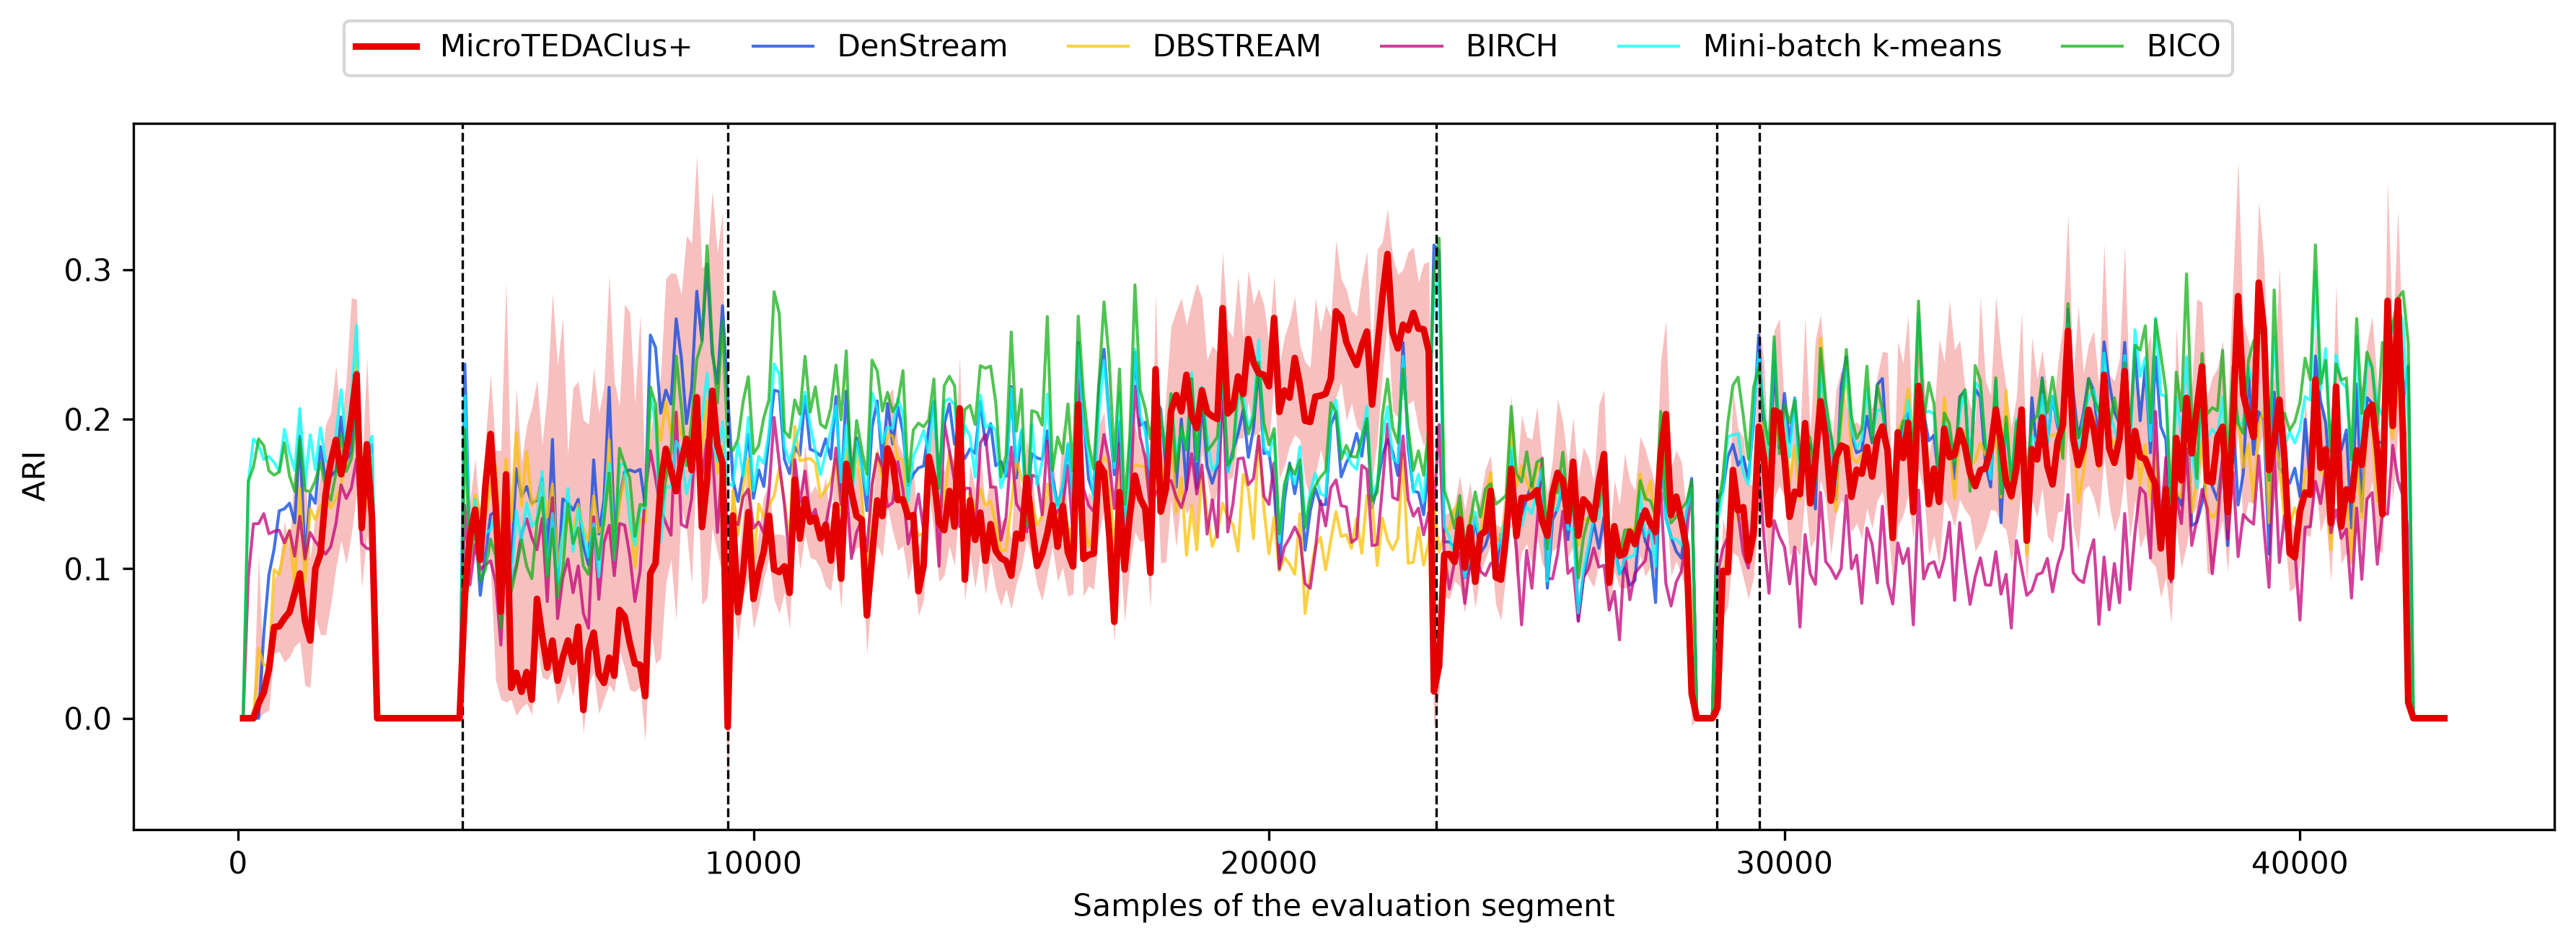
\includegraphics[width=\textwidth]{RealData/artifacts/plots/insects_abrupt.png}
    \caption[Batch ARI along the evaluation segment of \InsectsAbrupt]{Batch ARI of \MicroTEDAClusPlus and the benchmark models along the evaluation segment of \InsectsAbrupt, with the change points of the stream as dashed lines. Medians, with the interquartile band of \MicroTEDAClusPlus, over the 78 runs that every model finished.}
    \label{fig:real_insects_abrupt}
\end{figure}

\Cref{fig:real_insects_abrupt} follows the models along \InsectsAbrupt. \MicroTEDAClusPlus is neither consistently above nor below the benchmark models: it falls below all of them for a stretch after the first change point and rises above all of them for a stretch before the third. In three stretches the median ARI of every model is zero. They are batches of a single class (\cref{tab:real_single_class}), whose ARI is one for a model that placed the whole batch in one cluster and zero otherwise (\cref{subsec:real_order}).

\subsection{Cost}
\label{subsec:real_cost}

\begin{table}[htbp]
\centering
\small
\caption[Execution time and memory of \modelname{MicroTEDAClus+} and the benchmark models on the real datasets]{Execution time and memory of \modelname{MicroTEDAClus+} and the benchmark models on the real datasets: medians over 32 runs, except 28 in INS-A, 25 in INS-I, 26 in INS-R, 22 in GAS, 31 in KDD, 25 in PEN. A dash marks a model left out of a dataset, and every model of a dataset that leaves \MicroTEDAClusPlus{} out.}
\adjustbox{max width=\textwidth, max totalheight=0.82\textheight}{%
\begin{tabular}{l c c c c c c c c }
\toprule
Model & INS-A & INS-I & INS-R & GAS & KDD & COV & PEN & SHU \\
\midrule
\multicolumn{9}{l}{\textit{Learning time [ms]}} \\
\modelname{MicroTEDAClus+} & 5005 & 460 & 8780 & 225 & 2020 & - & 170 & 620 \\
Better/same/worse & 0/1/4 & 3/0/2 & 0/2/3 & 2/2/1 & 3/1/1 & - & 1/1/3 & 0/2/3 \\
\modelname{DenStream} & \textcolor{red}{770} & \textbf{890} & \textcolor{red}{1200} & \textbf{860} & \textbf{7240} & - & \textcolor{red}{90} & \textcolor{red}{220} \\
\modelname{DBSTREAM} & 3630 & \textbf{8770} & 6515 & \textbf{1210} & \textbf{38730} & - & \textbf{520} & 800 \\
\modelname{BIRCH} & \textcolor{red}{1325} & \textbf{1680} & 6715 & 410 & \textbf{12180} & - & 190 & 635 \\
\modelname{Mini-batch k-means} & \textcolor{red}{170} & \textcolor{red}{190} & \textcolor{red}{280} & \textcolor{red}{50} & 1910 & - & \textcolor{red}{30} & \textcolor{red}{185} \\
\modelname{BICO} & \textcolor{red}{130} & \textcolor{red}{150} & \textcolor{red}{210} & 270 & \textcolor{red}{1360} & - & \textcolor{red}{10} & \textcolor{red}{45} \\
\midrule
\multicolumn{9}{l}{\textit{Prediction time [ms]}} \\
\modelname{MicroTEDAClus+} & 65 & 30 & 130 & 20 & 270 & - & 10 & 40 \\
Better/same/worse & 4/1/0 & 5/0/0 & 4/1/0 & 4/1/0 & 5/0/0 & - & 4/1/0 & 5/0/0 \\
\modelname{DenStream} & \textbf{290} & \textbf{370} & \textbf{430} & \textbf{310} & \textbf{3070} & - & \textbf{70} & \textbf{70} \\
\modelname{DBSTREAM} & \textbf{665} & \textbf{310} & \textbf{1195} & \textbf{235} & \textbf{3270} & - & \textbf{110} & \textbf{120} \\
\modelname{BIRCH} & \textbf{230} & \textbf{260} & \textbf{545} & \textbf{75} & \textbf{2320} & - & \textbf{40} & \textbf{190} \\
\modelname{Mini-batch k-means} & 70 & \textbf{80} & 120 & 20 & \textbf{800} & - & 10 & \textbf{80} \\
\modelname{BICO} & \textbf{815} & \textbf{890} & \textbf{1040} & \textbf{240} & \textbf{7160} & - & \textbf{170} & \textbf{490} \\
\midrule
\multicolumn{9}{l}{\textit{Memory held at the end of the stream [KiB]}} \\
\modelname{MicroTEDAClus+} & 396 & 124 & 374 & 461 & 57 & - & 90 & 44 \\
Better/same/worse & 1/2/2 & 3/0/2 & 1/1/3 & 2/1/2 & 3/1/1 & - & 3/0/2 & 1/1/3 \\
\modelname{DenStream} & \textcolor{red}{65} & \textcolor{red}{88} & \textcolor{red}{49} & \textcolor{red}{262} & 62 & - & \textcolor{red}{57} & \textcolor{red}{7} \\
\modelname{DBSTREAM} & 256 & \textbf{722} & \textcolor{red}{224} & 378 & \textbf{295} & - & \textbf{219} & \textcolor{red}{20} \\
\modelname{BIRCH} & \textbf{600} & \textbf{829} & \textbf{1652} & \textbf{2058} & \textbf{475} & - & \textbf{146} & 58 \\
\modelname{Mini-batch k-means} & \textcolor{red}{8} & \textcolor{red}{8} & \textcolor{red}{8} & \textcolor{red}{26} & \textcolor{red}{7} & - & \textcolor{red}{9} & \textcolor{red}{6} \\
\modelname{BICO} & 612 & \textbf{592} & 224 & \textbf{946} & \textbf{412} & - & \textbf{155} & \textbf{94} \\
\midrule
\multicolumn{9}{l}{\textit{Peak memory [KiB]}} \\
\modelname{MicroTEDAClus+} & 12496 & 582 & 14556 & 928 & 231 & - & 1471 & 1562 \\
Better/same/worse & 0/0/5 & 1/3/1 & 0/1/4 & 2/2/1 & 4/0/1 & - & 0/0/5 & 0/0/5 \\
\modelname{DenStream} & \textcolor{red}{528} & 1450 & \textcolor{red}{834} & \textbf{4858} & \textbf{381} & - & \textcolor{red}{366} & \textcolor{red}{134} \\
\modelname{DBSTREAM} & \textcolor{red}{526} & 1016 & \textcolor{red}{472} & 1322 & \textbf{534} & - & \textcolor{red}{344} & \textcolor{red}{92} \\
\modelname{BIRCH} & \textcolor{red}{1774} & \textbf{2949} & 10368 & \textbf{3590} & \textbf{992} & - & \textcolor{red}{305} & \textcolor{red}{132} \\
\modelname{Mini-batch k-means} & \textcolor{red}{34} & \textcolor{red}{33} & \textcolor{red}{30} & \textcolor{red}{85} & \textcolor{red}{22} & - & \textcolor{red}{46} & \textcolor{red}{26} \\
\modelname{BICO} & \textcolor{red}{1208} & 1129 & \textcolor{red}{475} & 1714 & \textbf{612} & - & \textcolor{red}{301} & \textcolor{red}{226} \\
\bottomrule
\end{tabular}
}
\label{tab:real_cost}
\end{table}


\MicroTEDAClusPlus is faster than every benchmark model in the prediction stage of every dataset compared, or indistinguishable from one of them (\cref{tab:real_cost}). In the learning stage it is slower than \MiniBatchKMeans and \BICO in five of the seven datasets compared and than one of the two in the others, and faster than \DBSTREAM in four. The memory it holds at the end of the stream is smaller than that of some benchmark models and larger than that of others, and always larger than that of \MiniBatchKMeans. Its peak during the evaluation is the largest of all models in \InsectsAbrupt, \Pendigits and \Shuttle, and of all but \BIRCH in \InsectsReoccurring.

\section{Summary}
\label{sec:real_summary}

The real datasets add drifts that come from the conditions of the recording, classes that are not drawn from chosen distributions, and up to 128 dimensions. Evaluating on them required standardizing the features by the tuning segment, an order for each stream, search ranges widened and checked by a pilot, \MicroTEDAClusPlus without its noise label, and a limit on the tuning segment and on the size of the summaries. On them, \MicroTEDAClusPlus is better than every benchmark model in \Shuttle, worse than most of them in four datasets, and left out of \Covertype, where its summary exceeds the limit in most runs (\cref{tab:real_quality,tab:real_failures}). It predicts faster than the benchmark models, learns more slowly than the fastest of them, and reaches the largest peak of memory in three datasets (\cref{tab:real_cost}).
